%initialising document, adjust papersize, fontsize and page orientation to your needs
\documentclass[a4paper, fontsize = 8pt, landscape]{scrartcl}
\usepackage{../../../../misc_files/LateX/layout_and_colours}

\title{Web-Entwicklung}
\author{Jil Zerndt, Lucien Perret}
\date{December 2024}

\createtitlepagestyle
\createmainpagestyle
\begin{document}
\begin{multicols}{3}
	\thispagestyle{TitlePageStyle}
	\maketitle
	\begin{definition}{WEB-Architektur}
    \textbf{Client-Server-Modell:}
    \begin{itemize}
        \item Browser (Client) sendet Anfragen an Server
        \item Server verarbeitet Anfragen und sendet Antworten
        \item Kommunikation über HTTP/HTTPS (Port 80/443)
    \end{itemize}
    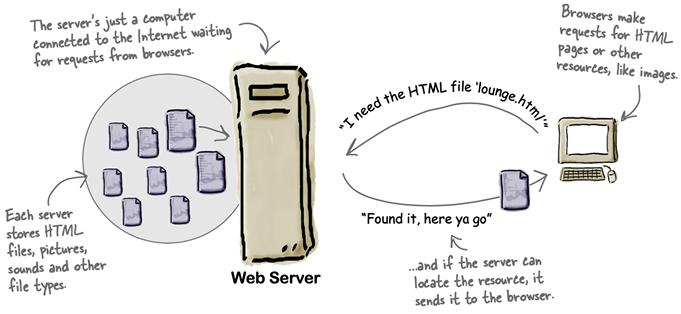
\includegraphics[width=1\linewidth]{images/web_architektur.png}
\end{definition}

\begin{concept}{Technologien}
    \textbf{Client-Seitig} $\rightarrow$ Front-end Entwickler
    \begin{itemize}
        \item Beschränkt auf Browser-Funktionalität
        \item Basistechnologien: HTML (Struktur), CSS (Darstellung), JavaScript (Verhalten)
        \item Browser APIs und Web-Standards
    \end{itemize}

    \textbf{Server-Seitig} $\rightarrow$ Back-end Entwickler
    \begin{itemize}
        \item Freie Wahl von Plattform und Programmiersprache
        \item Generiert Browser-kompatible Ausgabe
        \item Beispiele: Node.js, Express, REST APIs
    \end{itemize}
\end{concept}

\begin{concept}{Internet vs. WWW}
    \textbf{Internet:}
    \begin{itemize}
        \item Weltweites Netzwerk aus vielen Rechnernetzwerken
        \item Verschiedene Dienste: E-Mail, FTP, WWW, etc.
        \item Basis-Protokolle: TCP/IP
    \end{itemize}
    
    \textbf{World Wide Web:}
    \begin{itemize}
        \item Service, der auf dem Internet aufbaut
        \item Entwickelt von Tim Berners-Lee am CERN (1990er)
        \item Basiert auf: HTTP, HTML, URLs
    \end{itemize}
\end{concept}

\begin{concept}{Web-Standards}
    \begin{itemize}
        \item W3C (World Wide Web Consortium)
        \item WHATWG (Web Hypertext Application Technology Working Group)
        \item HTML Living Standard
        \item Browser-Hersteller (Chrome, Firefox, Safari, etc.)
    \end{itemize}
\end{concept}
	\raggedcolumns
	\section{JavaScript}

% Console and Data Types
\begin{formula}{Web-Konsole}
    JavaScript Console im Browser:
    \begin{itemize}
        \item \texttt{console.log(message)}: Gibt eine Nachricht aus
        \item \texttt{console.clear()}: Löscht die Konsole
        \item \texttt{console.trace(message)}: Stack trace ausgeben
        \item \texttt{console.error(message)}: stderr ausgeben
        \item \texttt{console.time()}: Timer starten
        \item \texttt{console.timeEnd()}: Timer stoppen
    \end{itemize}
    API-Dokumentation: \url{https://nodejs.org/api/console.html}
\end{formula}

\begin{definition}{Datentypen}
    JavaScript kennt folgende primitive Datentypen:
    \begin{itemize}
        \item \texttt{number}: 64-Bit Floating Point (IEEE 754)
        \begin{itemize}
            \item \texttt{Infinity}: $1/0$
            \item \texttt{NaN}: Not a Number ($0/0$)
        \end{itemize}
        \item \texttt{bigint}: Ganzzahlen beliebiger Größe (mit n am Ende)
        \item \texttt{string}: Zeichenketten in \texttt{''}, \texttt{""} oder \texttt{``}
        \item \texttt{boolean}: \texttt{true} oder \texttt{false}
        \item \texttt{undefined}: Variable deklariert aber nicht initialisiert
        \item \texttt{null}: Variable bewusst ohne Wert
        \item \texttt{symbol}: Eindeutiger Identifier
    \end{itemize}
\end{definition}

\begin{KR}{typeof-Operator}\\
Mit \texttt{typeof} kann der Typ eines Wertes ermittelt werden:
\begin{lstlisting}[language=JavaScript, style=basesmol]
typeof 42          // 'number'
typeof 42n         // 'bigint'
typeof "text"      // 'string'
typeof true        // 'boolean'
typeof undefined   // 'undefined'
typeof null        // 'object' (!)
typeof {}          // 'object'
typeof []          // 'object'
typeof (() => {})  // 'function'
typeof Infinity    // 'number'
typeof NaN         // 'number' !!
typeof 'number'    // 'string'
\end{lstlisting}
\end{KR}

\begin{theorem}{Variablenbindung}\\
    JavaScript kennt drei Arten der Variablendeklaration:
    \begin{itemize}
        \item \texttt{var}
        \begin{itemize}
            \item Scope: Funktions-Scope (Global oder Lokal)
            \item Eigenschaften: Kann neu deklariert werden
        \end{itemize}
        \item \texttt{let}
        \begin{itemize}
            \item Scope: Block-Scope (innerhalb von \{\})
            \item Eigenschaften: Moderne Variante für veränderliche Werte
        \end{itemize}
        \item \texttt{const}
        \begin{itemize}
            \item Scope: Block-Scope (innerhalb von \{\})
            \item Eigenschaften: Wert kann nicht neu zugewiesen werden
        \end{itemize}
    \end{itemize}
\end{theorem}

\begin{corollary}{Operatoren}
    \begin{itemize}
        \item Arithmetische Operatoren: $+, -, *, /, \%, ++, --$
        \item Zuweisungsoperatoren: $=, +=, -=, *=, /=, \%=, **=, $\\$<<=, >>=, >>>=, \&=, ^=, |=$
        \item Vergleichsoperatoren: $==, ===, !=, !==, >, <, >=, <=$
        \item Logische Operatoren: $\&\&, ||, !$
        \item Bitweise Operatoren: $\&, |, ^, ~, <<, >>, >>>$
        \item Sonstige Operatoren: \texttt{typeof}, \texttt{instanceof}
    \end{itemize}
\end{corollary}

\begin{formula}{Vergleichsoperatoren}
    JavaScript unterscheidet zwei Arten von Gleichheit:
    \begin{itemize}
        \item \texttt{==} und \texttt{!=}: Mit Typumwandlung
        \item \texttt{===} und \texttt{!==}: Ohne Typumwandlung (strikt)
    \end{itemize}
\begin{lstlisting}[language=JavaScript, style=basesmol]
5 == "5"     // true  (Typumwandlung)
5 === "5"    // false (keine Typumwandlung)
null == undefined    // true
null === undefined   // false
\end{lstlisting}
\end{formula}

\begin{KR}{Verzweigungen\text{,} Wiederholung und Switch Case}
    \begin{itemize}
        \item \texttt{if (condition) \{...\} else \{...\}}
        \item \texttt{switch (expression) \{ case x: ... break; default: ... \}}
        \item \texttt{for (initialization; condition; increment) \{...\}}
        \item \texttt{while (condition) \{...\}}
        \item \texttt{do \{...\} while (condition)}
        \item \texttt{for (let x of iterable) \{...\}}
    \end{itemize}
\end{KR}

% Control Structures
\begin{example2}{Kontrollstrukturen}
\begin{lstlisting}[language=JavaScript, style=basesmol]
// If-Statement
if (condition) {
    // code
} else if (otherCondition) {
    // code
} else {
    // code
}

// Switch Statement
switch(value) {
    case 1:
        // code
        break;
    case 2:
        // code
        break;
    default:
        // code
}

// Loops
for (let i = 0; i < n; i++) { }
while (condition) { }
do { } while (condition);
for (let item of array) { }
for (let key in object) { }
\end{lstlisting}
\end{example2}

\begin{KR}{Funktionsdefinition}
    \begin{itemize}
        \item \texttt{function name(parameters) \{...\}}
        \item \texttt{const name = (parameters) => \{...\}}
        \item \texttt{const name = parameters => \{...\}}
        \item \texttt{const name = parameters => expression}
    \end{itemize}
\end{KR}



% Functions
\begin{example2}{Funktionsdefinitionen}
JavaScript kennt verschiedene Arten, Funktionen zu definieren:
\begin{lstlisting}[language=JavaScript, style=basesmol]
// Funktionsdeklaration
function add(a, b) {
    return a + b;
}

// Funktionsausdruck
const multiply = function(a, b) {
    return a * b;
};

// Arrow Function
const subtract = (a, b) => a - b;

// Arrow Function mit Block
const divide = (a, b) => {
    if (b === 0) throw new Error('Division by zero');
    return a / b;
};
\end{lstlisting}
\end{example2}

\subsection{Objects and Arrays}

\begin{theorem}{Objekt vs Array}

    \begin{tabular}{|l|l|l|}
        \hline
        Was & Objekt & Array \\
        \hline
        Art & Attribut-Wert-Paare & Sequenz von Werten \\
        \hline
        Literalnotation & werte $=\{$ a: 1, b: 2$\}$ & liste $=[1,2,3]$ \\
        \hline
        Ohne Inhalt & werte $=\{ \}$ & liste $=[]$ \\
        \hline
        Elementzugriff & werte[''a'' $]$ oder werte.a & liste[0] \\
        \hline
        \end{tabular}
\end{theorem}

\begin{concept}{Json}
    JavaScript Object Notation
    \begin{itemize}
    \item Daten-Austauschformat, nicht nur für JavaScript
    \item Orientiert an Notation für JavaScript-Objektliterale
  \end{itemize}
  https://www.json.org/json-en.html
\begin{lstlisting}[language=JavaScript, style=basesmol]
> JSON.stringify({type: "cat", name: "Mimi", age: 3})
'{"type":"cat", "name":"Mimi", "age":3}'
> JSON.parse('{"type": "cat", "name": "Mimi", "age": 3}')
{type: 'cat', name: 'Mimi', age: 3}
\end{lstlisting}
\end{concept}

\begin{definition}{JS-Objekte}
    sind Sammlungen von Schlüssel-Wert-Paaren:
    \begin{itemize}
        \item Eigenschaften können dynamisch hinzugefügt/entfernt werden
        \item Werte können beliebige Typen sein (auch Funktionen)
        \item Schlüssel sind immer Strings oder Symbols
    \end{itemize}
\end{definition}

\begin{examplecode}{Objekte erstellen und manipulieren}
\begin{lstlisting}[language=JavaScript, style=basesmol]
// Objekt-Literal
const person = {
    name: "Alice",
    age: 30,
    greet() {
        return "Hello, I am" + this.name;
    }
};

// Eigenschaften manipulieren
person.job = "Developer";    // hinzufuegen
delete person.age;          // loeschen
"name" in person;           // true
\end{lstlisting}
\end{examplecode}

\begin{formula}{Arrays}
    Arrays in JavaScript sind spezielle Objekte für geordnete Sammlungen:
    \begin{itemize}
        \item \texttt{push()}, \texttt{pop()}: Ende hinzufügen/entfernen
        \item \texttt{unshift()}, \texttt{shift()}: Anfang hinzufügen/entfernen
        \item \texttt{splice()}: Elemente einfügen/entfernen
        \item \texttt{slice()}: Teilarray erstellen
        \item \texttt{map()}, \texttt{filter()}, \texttt{reduce()}: Funktional
        \item \texttt{forEach()}: Iteration über Elemente
        \item \texttt{indexOf()}, \texttt{lastIndexOf()}: Index suchen
        \item \texttt{concat()}: Arrays zusammenfügen
        \item \texttt{sort()}, \texttt{reverse()}: Sortieren/Umkehren
    \end{itemize}
\begin{lstlisting}[language=JavaScript, style=basesmol]
const arr = [1, 2, 3];
arr.push(4);             // [1,2,3,4]
arr.pop();              // [1,2,3]
arr.unshift(0);         // [0,1,2,3]
arr.shift();            // [1,2,3]
\end{lstlisting}

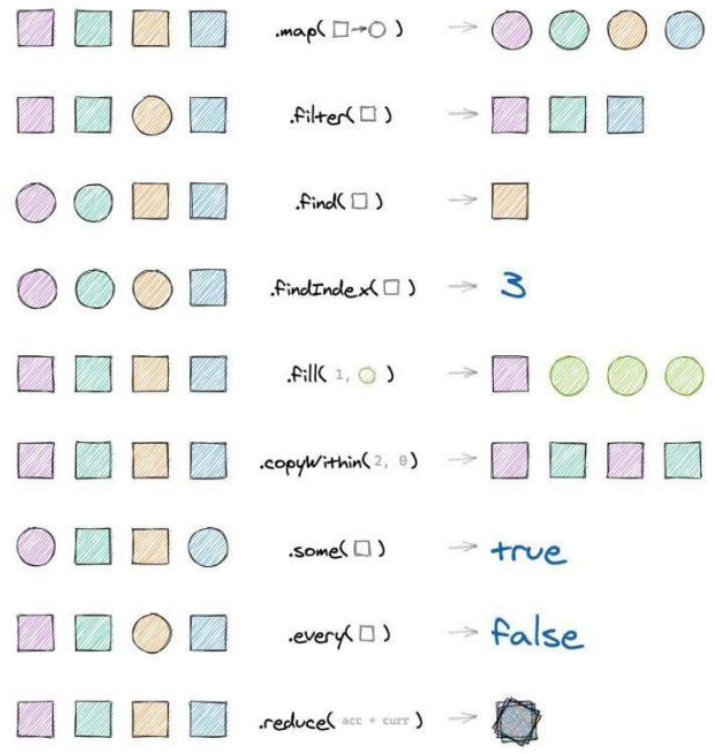
\includegraphics[width=0.5\linewidth]{images/array_cheatsheet.png}

\textcolor{red}{Achtung:} draw new!!!
\end{formula}
 
\subsection{Funktionen und funktionale Programmierung}

\begin{definition}{Funktionen}
    \begin{itemize}
        \item Funktionen sind spezielle, aufrufbare Objekte
        \item Man kann ihnen jederzeit Attribute oder Methoden hinzufügen
        \item Sie haben bereits vordefinierte Methoden
      \end{itemize}
\begin{lstlisting}[language=JavaScript, style=basesmol]
> const add = (x, y) => x + y
> add.doc = "This function adds two values"
> add(3,4)
7
> add.doc
'This function adds two values'
\end{lstlisting}
\end{definition}

\begin{concept}{Modulsystem in JavaScript}
    \begin{itemize}
        \item \texttt{import} und \texttt{export} für Module
        \item \texttt{export default} für Standardexport
        \item \texttt{import \{name\} from 'module'} für benannte Exports
        \item \texttt{import * as name from 'module'} für alle Exports
    \end{itemize}
\begin{lstlisting}[language=JavaScript, style=basesmol]
const car = {                   //car-lib.js
    brand: 'Ford',
    model: 'Fiesta'
}
module.exports = car
const car = require('./car-lib') //other js file
\end{lstlisting}
\end{concept}

\subsection{Prototypen von Objekten}

\begin{definition}{Prototypen}
    \begin{itemize}
        \item Die meisten Objekte haben ein Prototyp-Objekt.
        \item Dieses fungiert als Fallback für Attribute und Methoden.
      \end{itemize}
\begin{lstlisting}[language=JavaScript, style=basesmol, numbers=none, xleftmargin=-2pt]
>Object.getPrototypeOf(Math.max)==Function.prototype
true
>Object.getPrototypeOf([])==Array.prototype
true
>Object.getPrototypeOf(Function.prototype)==Object.prototype
true
>Object.getPrototypeOf(Array.prototype)==Object.prototype
true
\end{lstlisting}
\end{definition}

\begin{concept}{Prototypen-Kette}
    Call, apply, bind
    \begin{itemize}
        \item Weitere Argumente von call : Argumente der Funktion
        \item Weiteres Argument von apply : Array mit den Argumenten
        \item Erzeugt neue Funktion mit gebundenem this
    \end{itemize}
\begin{lstlisting}[language=JavaScript, style=basesmol]
function Employee (name, salary) {
    Person.call(this, name)
    this.salary = salary
}
Employee.prototype = new Person()
Employee.prototype.constructor = Employee
let e17 = new Employee("Mary", 7000)
console.log(e17.toString()) // Person with name 'Mary' 
console.log(e17.salary) // 7000 
\end{lstlisting}
\end{concept}

\begin{definition}{Klassen}
    \begin{itemize}
        \item Klassen sind syntaktischer Zucker für Prototypen
        \item Klassen können Attribute und Methoden enthalten
        \item Klassen können von anderen Klassen erben
    \end{itemize}
\begin{lstlisting}[language=JavaScript, style=basesmol]
class Person {
    constructor (name) {
        this.name = name
    }
    toString () {
        return `Person with name '${this.name}'
    }
}
let p35 = new Person("John")
console.log(p35.toString()) // Person with name 'John'
\end{lstlisting}
\end{definition}

\begin{code}{Vererbung}
\begin{lstlisting}[language=JavaScript, style=basesmol]
class Employee extends Person {
    constructor (name, salary) {
        super(name)
        this.salary = salary
    }
    toString () {
        return `${super.toString()} and salary ${this.salary}
    }
}
let e17 = new Employee("Mary", 7000);
console.log(e17.toString()) /* Person with name 'Mary' and salary 7000 */
console.log(e17.salary) /* 7000 */
\end{lstlisting}
\end{code}

\begin{examplecode}{Getter und Setter}
\begin{lstlisting}[language=JavaScript, style=basesmol]
class PartTimeEmployee extends Employee {
    constructor (name, salary, percentage) {
        super(name, salary)
        this.percentage = percentage
    }
    get salary100 () { return this.salary * 100 / this.percentage}
    set salary100 (amount) { this.salary = amount * this.percentage / 100 }
}
let e18 = new PartTimeEmployee("Bob", 4000, 50)
console.log(e18.salary100) /* -> 8000 */
e18.salary100 = 9000
console.log(e18.salary) /* \ 4500 */
\end{lstlisting}
\end{examplecode}


\subsubsection{Filesystem}

\begin{code}{Pfade der Datei}
Um Pfad-informationen einer Datei zu ermitteln muss man dies mit require('path') machen.
\begin{lstlisting}[language=JavaScript, style=basesmol]
const path = require('path')
const notes = '/users/bkrt/notes.txt'
path.dirname(notes) /* /users/bkrt */
path.basename(notes) /* notes.txt */
path.extname(notes) /* .txt */
path.basename(notes, path.extname(notes)) /* notes */
\end{lstlisting}
\end{code}

\begin{definition}{File API}
    Mit require('fs') wird auf die File-Api zugegriffen.
    Die File-Api bietet Funktionen zum Lesen und Schreiben von Dateien.
\end{definition}

\begin{formula}{FS Funktionen}
\begin{itemize}
    \item \texttt{fs.access}: Zugriff auf Datei oder Ordner prüfen
    \item \texttt{fs.mkdir}: Verzeichnis anlegen
    \item \texttt{fs.readdir}: Verzeichnis lesen, liefert Array von Einträgen
    \item \texttt{fs.rename}: Verzeichnis umbenennen
    \item \texttt{fs.rmdir}: Verzeichnis löschen
    \item \texttt{fs.chmod}: Berechtigungen ändern
    \item \texttt{fs.chown}: Besitzer und Gruppe ändern
    \item \texttt{fs.copyFile}: Datei kopieren
    \item \texttt{fs.link}: Besitzer und Gruppe ändern
    \item \texttt{fs.symlink}: Symbolic Link anlegen
    \item \texttt{fs.watchFile}: Datei auf Änderungen überwachen
\end{itemize}
\end{formula}

\begin{code}{Datei-Informationen}
\begin{lstlisting}[language=JavaScript, style=basesmol]
const fs = require('fs')
fs.stat('test.txt' , (err, stats) => {
    if (err) {
    console.error(err)
    return
    }
    stats.isFile() /* true */
    stats.isDirectory() /* false */
    stats.isSymbolicLink() /* false */
stats.size /* 1024000 = ca 1MB */
})
\end{lstlisting}
\end{code}

\begin{examplecode}{Dateien lesen und schreiben}
\begin{lstlisting}[language=JavaScript, style=basesmol]
const fs = require('fs')
fs.readFile('/etc/hosts',"utf8", (err, data) => {
        if (err) throw err
        console.log(data)
})

const content = 'Node was here!'
fs.writeFile('/Users/bkrt/test.txt', content, (err) => {
    if (err) {
        console.error(`Failed to write file: ${err}`)
        return
    } // file written successfully
})
\end{lstlisting}
\end{examplecode}

\subsection{Asynchrone Programmierung}

% Asynchronous Programming
\begin{concept}{Asynchrone Programmierung}\\
    JavaScript verwendet verschiedene Mechanismen für asynchrone Operationen:
    \begin{itemize}
        \item Callbacks: Traditioneller Ansatz
        \item Promises: Moderner Ansatz für strukturiertere asynchrone Operationen
        \item Async/Await: Syntaktischer Zucker für Promises
    \end{itemize}
\end{concept}

\subsubsection{Callbacks und Timers}

\begin{definition}{Callbacks}
Ein Callback ist eine Funktion, welche als Argument einer anderen Funktion übergeben wird und erst aufgerufen wird, wenn das Ereignis eingetreten ist. 
In der folgenden Abbildung wird die KlickFunktion vom Button mit der Id «Button» abonniert.
\begin{lstlisting}[language=JavaScript, style=basesmol]
document.getElementById('button').addEventListener('click', () => {
//item clicked
})
\end{lstlisting}
\end{definition}

\begin{code}{SetTimeout}
\begin{itemize}
  \item Mit setTimeout kann Code definiert werden, der zu einem späteren Zeitpunkt ausgeführt werden soll
  \item Eintrag in die Timer-Liste, auch wenn Zeit auf 0 gesetzt wird
  \item Kann mit clearTimeout entfernt werden
\end{itemize}
\begin{lstlisting}[language=JavaScript, style=basesmol]
setTimeout(() => {
    /* runs after 50 milliseconds */
}, 50)
\end{lstlisting}
\end{code}

\begin{code}{SetInterval}
\begin{itemize}
  \item Callback alle n Millisekunden in die Callback Queue eingefügt
  \item Kann mit clearInterval beendet werden
\end{itemize}
\begin{lstlisting}[language=JavaScript, style=basesmol]
const id = setInterval(() => {
// runs every 2 seconds
}, 2000)
clearInterval(id)
\end{lstlisting}
\end{code}

\begin{code}{SetImmediate}
\begin{itemize}
  \item Callback wird in die Immediate Queue eingefügt
  \item Wird nach dem aktuellen Event-Loop ausgeführt
\end{itemize}
\begin{lstlisting}[language=JavaScript, style=basesmol]
setImmediate(() => {
    console.log('immediate')
})
\end{lstlisting}
\end{code}

\subsubsection{Events und Promises}

\begin{definition}{Event-Modul (EventMitter)}
\begin{itemize}
  \item EventEmitter verwaltet Liste von Listeners zu bestimmten Events
  \item Listener für das Event können hinzugefügt oder entfernt werden
  \item Event kann ausgelöst werden $\rightarrow$ Listener werden informiert
\end{itemize}
\end{definition}

\begin{examplecode}{Listener hinzufügen}
\begin{lstlisting}[language=JavaScript, style=basesmol]
const EventEmitter = require('events')
const door = new EventEmitter()

door.on('open', () => {
    console.log('Door was opened')
})
\end{lstlisting}
\end{examplecode}

\begin{examplecode}{Event auslösen}
\begin{lstlisting}[language=JavaScript, style=basesmol]
door.on('open', (speed) => {
    console.log(`Door was opened, speed: ${speed || 'unknown'}`)
})

door.emit('open')
door.emit('open', 'slow')
\end{lstlisting}
\end{examplecode}

\begin{definition}{Promises}
Ist ein Platzhalter für einen Wert, der erst später voraussichtlich verfügbar sein wird.
Funktion mit Promise:
\begin{lstlisting}[language=JavaScript, style=basesmol]
function readFilePromise(file) {
    let promise = new Promise(function resolver(resolve, reject) {
        fs.readFile(file, "utf8", (err, data) => {
            if (err) reject(err);
            else resolve(data);
        });
    });
    return promise;
}
\end{lstlisting}
Gibt nun ein Promise-Object zurück
\end{definition}

\begin{concept}{Promise-Konstruktor erhält resolver-Funktion}

Rückgabe einer Promise: potentieller Wert kann später erfüllt oder zurückgewiesen werden
\begin{itemize}
  \item Rückgabe einer Promise: potentieller Wert
  \item kann später erfüllt oder zurückgewiesen werden
\end{itemize}
Aufruf neu:
\begin{lstlisting}[language=JavaScript, style=basesmol]
readFilePromise('/etc/hosts')
    .then(console.log)
    .catch(() => {
        console.log("Error reading file")
    })
\end{lstlisting}
\end{concept}

\begin{theorem}{Promise-Zustände}
\begin{itemize}
  \item pending: Ausgangzustand
  \item fulfilled: erfolgreich abgeschlossen
  \item rejected: ohne Erfolg abgeschlossen
  \end{itemize}
  Nur ein Zustandsübergang möglich und Zustand in Promise-Objekt gekapselt\\
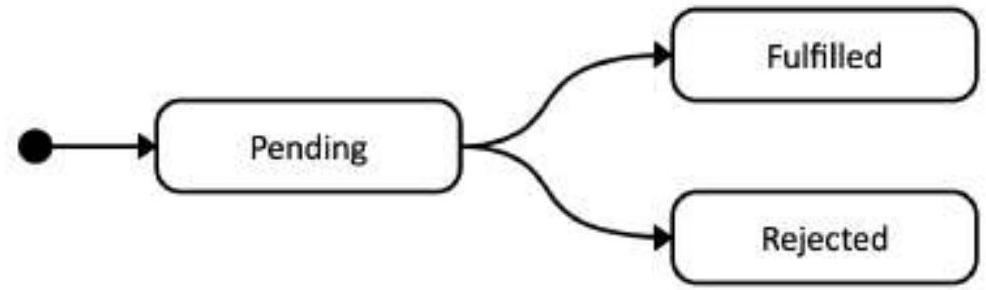
\includegraphics[width=0.8\linewidth]{images/2024_12_29_858f09cde51177c71657g-14}
\end{theorem}

\begin{corollary}{Promises Verknüpfen}
\begin{itemize}
  \item Then-Aufruf gibt selbst Promise zurück
  \item Catch-Aufruf ebenfalls, per Default erfüllt
  \item So können diese Aufrufe verkettet werden
  \item Promise, welche unmittelbar resolved wird: Promise.resolve (...)
  \item Promise, welche unmittelbar rejected wird: Promise.reject (...)
\end{itemize}
\end{corollary}

\begin{definition}{Promise.all()}
\begin{itemize}
  \item Erhält Array von Promises
  \item Erfüllt mit Array der Result, wenn alle erfüllt sind
  \item Zurückgewiesen sobald eine Promise zurückgewiesen wird
\end{itemize}
\end{definition}

\begin{definition}{Promise.race()}
\begin{itemize}
  \item Erhält Array von Promises
  \item Erfüllt sobald eine davon erfüllt ist
  \item Zurückgewiesen sobald eine davon zurückgewiesen wird
\end{itemize}
\end{definition}

\begin{code}{ASYNC/AWAIT}
\begin{lstlisting}[language=JavaScript, style=basesmol]
/* Bekanntes Beispiel */
const readHosts =() => {
    readFilePromise('/etc/hosts')
        .then(console.log)
        . catch(() => {
            console.log("Error reading file")
        })
}
/* Mit async/await */
const readHosts = async () => {
    try {
        console.log(await readFilePromise('/etc/hosts'))
    }
    catch (err) {
        console.log("Error reading file")
    }
}
\end{lstlisting}
Beispiel 2:
\begin{lstlisting}[language=JavaScript, style=basesmol]
function resolveAfter2Seconds (x) {
    return new Promise(resolve => {
        setTimeout(() => {
            resolve(x)
        }, 2000)
    })
}
async function add1(x) {
    var a = resolveAfter2Seconds(20)
    var b = resolveAfter2Seconds(30)
    return x + await a + await b
}
add1(10).then(console.log)
\end{lstlisting}
\end{code}

\begin{KR}{Promise Erstellung und Verwendung}
\begin{lstlisting}[language=JavaScript, style=basesmol]
// Promise erstellen
const myPromise = new Promise((resolve, reject) => {
    // Asynchrone Operation
    setTimeout(() => {
        if (/* erfolg */) {
            resolve(result);
        } else {
            reject(error);
        }
    }, 1000);
});

// Promise verwenden
myPromise
    .then(result => {
        // Erfolgsfall
    })
    .catch(error => {
        // Fehlerfall
    })
    .finally(() => {
        // Wird immer ausgefuhrt
    });

// Async/Await Syntax
async function myAsync() {
    try {
        const result = await myPromise;
        // Erfolgsfall
    } catch (error) {
        // Fehlerfall
    }
}
\end{lstlisting}
\end{KR}

% Modules and Node.js
\begin{concept}{Module System}
    JavaScript verwendet verschiedene Modulsysteme:
    \begin{itemize}
        \item CommonJS (Node.js): \texttt{require}/\texttt{module.exports}
        \item ES Modules: \texttt{import}/\texttt{export}
    \end{itemize}
\end{concept}

\begin{KR}{Module Import/Export}
\begin{lstlisting}[language=JavaScript, style=basesmol]
// CommonJS (Node.js)
const fs = require('fs');
module.exports = { /* ... */ };

// ES Modules
import { function1, function2 } from './module.js';
export const variable = 42;
export default class MyClass { /* ... */ }
\end{lstlisting}
\end{KR}

% Error Handling
\begin{KR}{Error Handling}
\begin{lstlisting}[language=JavaScript, style=basesmol]
try {
    // Code der Fehler werfen konnte
    throw new Error('Something went wrong');
} catch (error) {
    // Fehlerbehandlung
    console.error(error.message);
} finally {
    // Wird immer ausgefuhrt
    cleanup();
}
\end{lstlisting}
\end{KR}

\subsection{Webserver}
Die Standard-Ports von einem Webserver sind 80 und 443. Der Webserver wartet auf eine Anfrage vom Client.

\begin{definition}{Server im Internet}
\begin{itemize}
  \item Wartet auf Anfragen auf bestimmtem Port
  \item Client stellt Verbindung her und sendet Anfrage
  \item Server beantwortet Anfrage
\end{itemize}
\end{definition}

\begin{corollary}{Ports}
\begin{center}
\begin{tabular}{|l|l|}
\hline
Port & Service \\
\hline
$\mathbf{2 0}$ & FTP - Data \\
\hline
$\mathbf{2 1}$ & FTP - Control \\
\hline
$\mathbf{2 2}$ & SSH Remote Login Protocol \\
\hline
$\mathbf{2 3}$ & Telnet \\
\hline
$\mathbf{2 5}$ & Simple Mail Transfer Protocol (SMTP) \\
\hline
$\mathbf{5 3}$ & Domain Name System (DNS) \\
\hline
$\mathbf{8 0}$ & HTTP \\
\hline
$\mathbf{4 4 3}$ & HTTPs \\
\hline
\end{tabular}
\end{center}
\end{corollary}

\begin{definition}
    {File-Transfer} File Server\\
    Um Dateien auf einem File-Server auszutauschen, werden die Protokolle FTP (File Transfer Protocol) und SFTP (SSH File Transfer Protocol) verwendet.
\end{definition}

\subsubsection{HTTP}

\begin{theorem}{HTTP-Requests}
    \begin{itemize}
        \item GET: Ressource laden
        \item POST: Informationen senden
        \item PUT: Ressource anlegen, überschreiben
        \item PATCH: Ressource anpassen
        \item DELETE: Ressource löschen
    \end{itemize}
\end{theorem}

\begin{corollary}{HTTP-Response Codes}
    \begin{center}
    \begin{tabular}{|l|l|}
    \hline
    Code & Beschreibung \\
    \hline
    $\mathbf{1 x x}$ & Information (101 Switching protocols) \\
    \hline
    $\mathbf{2 x x}$ & Erfolg (200 OK) \\
    \hline
    $\mathbf{3 x x}$ & Weiterleitung (301 Moved permanently) \\
    \hline
    $\mathbf{4 x x}$ & Fehler in Anfrage (403 Forbidden, 404 Not Found) \\
    \hline
    $\mathbf{5 x x}$ & Server-Fehler (501 Not implemented) \\
    \hline
    \end{tabular}
    \end{center}
\end{corollary}

\columnbreak

\subsection{Einfacher Webserver (Node.js)}

\begin{concept}{Node.js Webserver}
\begin{lstlisting}[language=JavaScript, style=basesmol]
const {createServer} = require("http")
Let server = createServer((request, response) => {
    response.writeHead(200, {"Content-Type": "text/html"})
    response.write(`
        <h1>Hello!</h1>
        <p>You asked for <code>${request.url}</code></p>`)
    response.end()
})
server.listen(8000)
console.log("Listening! (port 8000)")|
\end{lstlisting}
\end{concept}


\begin{code}{Einfacher Webclient}
\begin{lstlisting}[language=JavaScript, style=basesmol]
const {request} = require("http")
let requestStream = request({
    hostname: "eloquentjavascript.net",
        path: "/20_node.html",
        method: "GET"
        headers: {Accept: "text/html"}
}, response => {
        console.log("Server responded with status code", response.statusCode)
})
requestStream.end()
\end{lstlisting}
\end{code}

\begin{examplecode}{Server und Client mit Streams}
\begin{lstlisting}[language=JavaScript, style=basesmol]
const {createServer} = require("http")
createServer((request, response) => {
    response.writeHead(200, {"Content-Type": "text/plain"})
        request.on("data", chunk =>
            response.write(chunk.toString().toUpperCase()))
        request.on("end" , () => response.end())
    }).listen(8000)
\end{lstlisting}

\begin{lstlisting}[language=JavaScript, style=basesmol]
const {request} = require("http")
Let rq = request({
    hostname: "localhost",
    port: 8000,
    method: "POST"
}, response => {
    response.on("data", chunk =>
    process.stdout.write(chunk.toString()));
})
rq.write("Hello server\n")
rq.write("And good bye\n")
rq.end()
\end{lstlisting}
\end{examplecode}

\begin{definition}{REST API}
\begin{itemize}
  \item REST: Representational State Transfer
  \item Zugriff auf Ressourcen über ihre Adresse (URI)
  \item Kein Zustand: jede Anfrage komplett unabhängig
  \item Kein Bezug zu vorhergehenden Anfragen
  \item Alle nötigen Informationen in Anfrage enthalten
  \item Verwenden der HTTP-Methoden: GET , PUT , POST , ...
\end{itemize}
\end{definition}

\begin{concept}{Express.js}\\
    Express.js ist ein minimales, aber flexibles Framework für Web-apps. Es hat zahlreiche Utilities und Erweiterungen. 
    Express.js basiert auf Node.js.
    $\rightarrow$ http://expressjs.com
\end{concept}


\begin{KR}{Installation}
\begin{itemize}
  \item Der Schritt npm init fragt eine Reihe von Informationen (Projektname, Version, ...) zum Projekt ab
  \item Als Entry Point ist hier index.js voreingestellt
  \item Das kann zum Beispiel in app.js geändert werden.
\end{itemize}
\begin{lstlisting}[language=JavaScript, style=basesmol]
$ mkdir myapp
$ cd myapp
$ npm init
$ npm install express --save
\end{lstlisting}
\end{KR}

\begin{code}{Beispiel: Express Server}
\begin{lstlisting}[language=JavaScript, style=basesmol]
const express = require('express')
const app = express()
const port = 3000
app.get('/', (req, res) => {
        res.send('Hello World!')
})
app.listen(port, () => {
    console.log(`Example app listening at http://localhost:${port}`)
}})
\end{lstlisting}
\end{code}

\begin{KR}{Routing}
\begin{lstlisting}[language=JavaScript, style=basesmol]
app.get('/', function (req, res) {
    res.send('Hello World!')
})
app.post('/', function (req, res) {
    res.send('Got a POST request')
})
app.put('/user', function (req, res) {
    res.send('Got a PUT request at /user')
})
app.delete('/user', function (req, res) {
    res.send('Got a DELETE request at /user')
})
\end{lstlisting}
\end{KR}






\subsection{Jasmine (Testing)}

\begin{examplecode}{Beispiel (zugehörige Tests)}
\begin{lstlisting}[language=JavaScript, style=basesmol]
/* PlayerSpec.js - Auszug */
describe("when song has been paused", function() {
    beforeEach(function() {
        player.play(song)
        player.pause()
    })
    it("should indicate that the song is currently paused", function() {
        expect(player.isPlaying).toBeFalsy()
        /* demonstrates use of 'not' with a custom matcher */
        expect(player).not.toBePlaying(song)
    })
    it("should be possible to resume", function() {
        player.resume()
        expect(player.isPlaying).toBeTruthy()
        expect(player.currentlyPlayingSong) .toEqual(song)
    })
})
\end{lstlisting}
\end{examplecode}

\begin{code}{JASMINE: MATCHER}
\begin{lstlisting}[language=JavaScript, style=basesmol]
expect([1, 2, 3]).toEqual([1, 2, 3])
expect(12).toBeTruthy()
expect("").toBeFalsy()
expect("Hello planet").not.toContain("world")
expect(null).toBeNull()
expect(8).toBeGreaterThan(5)
expect(12.34).toBeCloseTo(12.3, 1)
expect("horse_ebooks.jpg") .toMatch(/\w+.(jpg|gif|png|svg)/i)
\end{lstlisting}
\end{code}

\begin{KR}{JASMINE: TESTS DURCHFÜHREN}
\begin{lstlisting}[language=bash, style=basesmol]
$ npx jasmine
Randomized with seed 03741
Started
......
5 specs, 0 failures
Finished in 0.014 seconds
Randomized with seed 03741 
    (jasmine --random=true --seed=03741)
\end{lstlisting}
\end{KR}
    \section{Browser APIs und DOM}

\subsection{Vordefinierte Objekte}

\begin{definition}{Browser Objekte}
    Im Browser stehen spezielle globale Objekte zur Verfügung:
    \begin{itemize}
        \item \texttt{window}: Browserfenster und globaler Scope
        \item \texttt{document}: Das aktuelle HTML-Dokument
        \item \texttt{navigator}: Browser-Informationen
        \item \texttt{location}: URL-Informationen
        \item \texttt{history}: Browser-Verlauf
    \end{itemize}
\end{definition}

\begin{concept}{Document Object Model (DOM)}
    Das DOM ist eine Baumstruktur, die das HTML-Dokument repräsentiert:
    \begin{itemize}
        \item Jeder HTML-Tag wird zu einem Element-Knoten
        \item Text innerhalb von Tags wird zu Text-Knoten
        \item Attribute werden zu Attribut-Knoten
        \item Kommentare werden zu Kommentar-Knoten
    \end{itemize}
\end{concept}

\begin{KR}{DOM Navigation}
Zugriff auf DOM-Elemente:
\begin{lstlisting}[language=JavaScript, style=basesmol]
// Element ueber ID finden
const elem = document.getElementById('myId');

// Elemente ueber CSS-Selektor finden
const elem1 = document.querySelector('.myClass');
const elems = document.querySelectorAll('div.myClass');

// Navigation im DOM-Baum
elem.parentNode          // Elternknoten
elem.childNodes         // Alle Kindknoten
elem.children           // Nur Element-Kindknoten
elem.firstChild         // Erster Kindknoten
elem.lastChild          // Letzter Kindknoten
elem.nextSibling        // Naechster Geschwisterknoten
elem.previousSibling    // Vorheriger Geschwisterknoten
\end{lstlisting}
\end{KR}

\begin{KR}{DOM Manipulation}
Elemente erstellen und manipulieren:
\begin{lstlisting}[language=JavaScript, style=basesmol]
// Neues Element erstellen
const newDiv = document.createElement('div');
const newText = document.createTextNode('Hello');
newDiv.appendChild(newText);

// Element einfuegen
parentElem.appendChild(newDiv);
parentElem.insertBefore(newDiv, referenceElem);

// Element entfernen
elem.remove();
parentElem.removeChild(elem);

// Attribute manipulieren
elem.setAttribute('class', 'myClass');
elem.getAttribute('class');
elem.removeAttribute('class');

// HTML/Text Inhalt
elem.innerHTML = '<span>Text</span>';
elem.textContent = 'Nur Text';
\end{lstlisting}
\end{KR}

\subsection{Events}

\begin{concept}{Event Handling}
    Events sind Ereignisse, die im Browser auftreten:
    \begin{itemize}
        \item Benutzerinteraktionen (Klicks, Tastatureingaben)
        \item DOM-Änderungen
        \item Ressourcen laden
        \item Timer
    \end{itemize}
\end{concept}

\begin{KR}{Event Listener}
Event Listener registrieren und entfernen:
\begin{lstlisting}[language=JavaScript, style=basesmol]
// Event Listener hinzufuegen
element.addEventListener('click', function(event) {
    console.log('Clicked!', event);
});

// Mit Arrow Function
element.addEventListener('click', (event) => {
    console.log('Clicked!', event);
});

// Event Listener entfernen
const handler = (event) => {
    console.log('Clicked!', event);
};
element.addEventListener('click', handler);
element.removeEventListener('click', handler);
\end{lstlisting}
\end{KR}

\begin{formula}{Wichtige Event-Typen}
    \begin{itemize}
        \item Maus: \texttt{click}, \texttt{dblclick}, \texttt{mousedown}, \texttt{mouseup}, \texttt{mousemove}
        \item Tastatur: \texttt{keydown}, \texttt{keyup}, \texttt{keypress}
        \item Formular: \texttt{submit}, \texttt{change}, \texttt{input}, \texttt{focus}, \texttt{blur}
        \item Dokument: \texttt{DOMContentLoaded}, \texttt{load}, \texttt{unload}
        \item Fenster: \texttt{resize}, \texttt{scroll}
    \end{itemize}
\end{formula}

\begin{code}{Event Bubbling und Capturing}
\begin{lstlisting}[language=JavaScript, style=basesmol]
// Bubbling (default)
element.addEventListener('click', handler);

// Capturing
element.addEventListener('click', handler, true);

// Event-Ausbreitung stoppen
element.addEventListener('click', (event) => {
    event.stopPropagation();
});

// Default-Verhalten verhindern
element.addEventListener('click', (event) => {
    event.preventDefault();
});
\end{lstlisting}
\end{code}

\subsection{Browser Storage}

\begin{definition}{Storage APIs}
    Browser bieten verschiedene Möglichkeiten zur Datenspeicherung:
    \begin{itemize}
        \item \texttt{localStorage}: Permanente Speicherung
        \item \texttt{sessionStorage}: Temporäre Speicherung (nur für aktuelle Session)
        \item \texttt{cookies}: Kleine Datenpakete, die auch zum Server gesendet werden
        \item \texttt{indexedDB}: NoSQL-Datenbank im Browser
    \end{itemize}
\end{definition}

\begin{KR}{LocalStorage Verwendung}
\begin{lstlisting}[language=JavaScript, style=basesmol]
// Daten speichern
localStorage.setItem('key', 'value');
localStorage.setItem('user', JSON.stringify({
    name: 'John',
    age: 30
}));

// Daten abrufen
const value = localStorage.getItem('key');
const user = JSON.parse(localStorage.getItem('user'));

// Daten loeschen
localStorage.removeItem('key');
localStorage.clear();  // Alles loeschen
\end{lstlisting}
\end{KR}

\subsection{Canvas und SVG}

\begin{concept}{Grafik im Browser}
    Zwei Haupttechnologien für Grafiken:
    \begin{itemize}
        \item Canvas: Pixel-basierte Grafik
        \item SVG: Vektor-basierte Grafik
    \end{itemize}
\end{concept}

\begin{KR}{Canvas Grundlagen}
\begin{lstlisting}[language=JavaScript, style=basesmol]
const canvas = document.querySelector('canvas');
const ctx = canvas.getContext('2d');

// Rechteck zeichnen
ctx.fillStyle = 'red';
ctx.fillRect(10, 10, 100, 50);

// Pfad zeichnen
ctx.beginPath();
ctx.moveTo(10, 10);
ctx.lineTo(50, 50);
ctx.stroke();

// Text zeichnen
ctx.font = '20px Arial';
ctx.fillText('Hello', 10, 50);
\end{lstlisting}
\end{KR}

\begin{KR}{SVG Manipulation}
\begin{lstlisting}[language=JavaScript, style=basesmol]
// SVG-Element erstellen
const svg = document.createElementNS(
    "http://www.w3.org/2000/svg", 
    "svg"
);
svg.setAttribute("width", "100");
svg.setAttribute("height", "100");

// Kreis hinzufuegen
const circle = document.createElementNS(
    "http://www.w3.org/2000/svg", 
    "circle"
);
circle.setAttribute("cx", "50");
circle.setAttribute("cy", "50");
circle.setAttribute("r", "40");
circle.setAttribute("fill", "red");

svg.appendChild(circle);
\end{lstlisting}
\end{KR}

    \section{Client-Server Interaktion}

\subsection{Formulare}

\begin{definition}{HTML-Formulare}
    Formulare ermöglichen Benutzereingaben und Datenübertragung:
    \begin{itemize}
        \item \texttt{<form>} Element mit \texttt{action} und \texttt{method}
        \item \texttt{method="GET"}: Daten in URL (sichtbar)
        \item \texttt{method="POST"}: Daten im Request-Body (unsichtbar)
        \item Verschiedene Input-Typen: text, password, checkbox, radio, etc.
    \end{itemize}
\end{definition}

\begin{KR}{Formular Handling}
\begin{lstlisting}[language=HTML, style=basesmol]
<!-- HTML Form -->
<form action="/submit" method="POST">
    <label for="username">Username:</label>
    <input type="text" id="username" name="username">
    
    <label for="password">Password:</label>
    <input type="password" id="password" name="password">
    
    <button type="submit">Login</button>
</form>

<!-- JavaScript Handler -->
form.addEventListener('submit', (event) => {
    event.preventDefault(); // Verhindert Standard-Submit
    
    const formData = new FormData(form);
    // Zugriff auf Formular-Daten
    const username = formData.get('username');
    const password = formData.get('password');
});
\end{lstlisting}
\end{KR}

\begin{formula}{Formular Events}
    Wichtige Events bei Formularen:
    \begin{itemize}
        \item \texttt{submit}: Formular wird abgeschickt
        \item \texttt{reset}: Formular wird zurückgesetzt
        \item \texttt{change}: Wert eines Elements wurde geändert
        \item \texttt{input}: Wert wird gerade geändert
        \item \texttt{focus}: Element erhält Fokus
        \item \texttt{blur}: Element verliert Fokus
    \end{itemize}
\end{formula}

\subsection{AJAX und Fetch API}

\begin{concept}{AJAX}
    Asynchronous JavaScript And XML:
    \begin{itemize}
        \item Asynchrone Kommunikation mit dem Server
        \item Kein vollständiges Neuladen der Seite nötig
        \item Moderne Alternative: Fetch API
        \item Datenformate: JSON, XML, Plain Text
    \end{itemize}
\end{concept}

\begin{KR}{Fetch API Grundlagen}
\begin{lstlisting}[language=JavaScript, style=basesmol]
// GET Request
fetch('https://api.example.com/data')
    .then(response => response.json())
    .then(data => console.log(data))
    .catch(error => console.error('Error:', error));

// POST Request
fetch('https://api.example.com/data', {
    method: 'POST',
    headers: {
        'Content-Type': 'application/json',
    },
    body: JSON.stringify({
        key: 'value'
    })
})
    .then(response => response.json())
    .then(data => console.log(data));

// Mit async/await
async function fetchData() {
    try {
        const response = await fetch('https://api.example.com/data');
        const data = await response.json();
        console.log(data);
    } catch (error) {
        console.error('Error:', error);
    }
}
\end{lstlisting}
\end{KR}

\subsection{Cookies und Sessions}

\begin{definition}{Cookies}
    HTTP-Cookies sind kleine Datenpakete:
    \begin{itemize}
        \item Werden vom Server gesetzt
        \item Im Browser gespeichert
        \item Bei jedem Request mitgesendet
        \item Haben Name, Wert, Ablaufdatum und Domain
    \end{itemize}
\end{definition}

\begin{KR}{Cookie Handling}
\begin{lstlisting}[language=JavaScript, style=basesmol]
// Cookie setzen
document.cookie = "username=John Doe; expires=Thu, 18 Dec 2024 12:00:00 UTC; path=/";

// Cookie lesen
const cookies = document.cookie.split(';').reduce((acc, cookie) => {
    const [name, value] = cookie.trim().split('=');
    acc[name] = value;
    return acc;
}, {});

// Cookie loeschen
document.cookie = "username=; expires=Thu, 01 Jan 1970 00:00:00 UTC; path=/;";
\end{lstlisting}
\end{KR}

\begin{concept}{Sessions}
    Server-seitige Speicherung von Benutzerdaten:
    \begin{itemize}
        \item Session-ID wird in Cookie gespeichert
        \item Daten bleiben auf dem Server
        \item Sicherer als Cookies für sensible Daten
        \item Temporär (bis Browser geschlossen wird)
    \end{itemize}
\end{concept}

\subsection{REST APIs}

\begin{definition}{REST Prinzipien}
    Representational State Transfer:
    \begin{itemize}
        \item Zustandslos (Stateless)
        \item Ressourcen-orientiert
        \item Einheitliche Schnittstelle
        \item Standard HTTP-Methoden
    \end{itemize}
\end{definition}

\begin{theorem}{HTTP-Methoden}
    \begin{center}
    \begin{tabular}{|l|l|}
    \hline
    Methode & Verwendung \\
    \hline
    GET & Daten abrufen \\
    \hline
    POST & Neue Daten erstellen \\
    \hline
    PUT & Daten aktualisieren (komplett) \\
    \hline
    PATCH & Daten aktualisieren (teilweise) \\
    \hline
    DELETE & Daten löschen \\
    \hline
    \end{tabular}
    \end{center}
\end{theorem}

\begin{KR}{REST API Implementierung mit Express}
\begin{lstlisting}[language=JavaScript, style=basesmol]
const express = require('express');
const app = express();
app.use(express.json());

// GET - Alle Benutzer abrufen
app.get('/api/users', (req, res) => {
    res.json(users);
});

// GET - Einzelnen Benutzer abrufen
app.get('/api/users/:id', (req, res) => {
    const user = users.find(u => u.id === parseInt(req.params.id));
    if (!user) return res.status(404).send('User not found');
    res.json(user);
});

// POST - Neuen Benutzer erstellen
app.post('/api/users', (req, res) => {
    const user = {
        id: users.length + 1,
        name: req.body.name
    };
    users.push(user);
    res.status(201).json(user);
});

// PUT - Benutzer aktualisieren
app.put('/api/users/:id', (req, res) => {
    const user = users.find(u => u.id === parseInt(req.params.id));
    if (!user) return res.status(404).send('User not found');
    
    user.name = req.body.name;
    res.json(user);
});

// DELETE - Benutzer loeschen
app.delete('/api/users/:id', (req, res) => {
    const user = users.find(u => u.id === parseInt(req.params.id));
    if (!user) return res.status(404).send('User not found');
    
    const index = users.indexOf(user);
    users.splice(index, 1);
    res.json(user);
});
\end{lstlisting}
\end{KR}

\begin{corollary}{HTTP Status Codes}
    \begin{center}
    \begin{tabular}{|l|l|}
    \hline
    Code & Bedeutung \\
    \hline
    200 & OK - Erfolgreich \\
    \hline
    201 & Created - Ressource erstellt \\
    \hline
    400 & Bad Request - Fehlerhafte Anfrage \\
    \hline
    401 & Unauthorized - Nicht authentifiziert \\
    \hline
    403 & Forbidden - Keine Berechtigung \\
    \hline
    404 & Not Found - Ressource nicht gefunden \\
    \hline
    500 & Internal Server Error - Serverfehler \\
    \hline
    \end{tabular}
    \end{center}
\end{corollary}

    \section{UI-Bibliotheken und Komponenten}

\subsection{Frameworks und Bibliotheken}

\begin{definition}{Framework vs. Bibliothek}
    \begin{itemize}
        \item \textbf{Bibliothek}: Kontrolle beim eigenen Programm, Funktionen werden nach Bedarf verwendet
        \item \textbf{Framework}: Rahmen für die Anwendung, Kontrolle liegt beim Framework ("Hollywood-Prinzip")
    \end{itemize}
\end{definition}

\begin{concept}{Komponenten-basierte Entwicklung}
    Grundprinzipien:
    \begin{itemize}
        \item UI wird in wiederverwendbare Komponenten aufgeteilt
        \item Komponenten können verschachtelt werden
        \item Datenfluss von oben nach unten (props)
        \item Zustand wird in Komponenten verwaltet
        \item Deklarativer Ansatz: UI als Funktion des Zustands
    \end{itemize}
\end{concept}

\subsection{JSX und SJDON}

\begin{definition}{JSX}
    JSX ist eine Erweiterung der JavaScript-Syntax:
    \begin{itemize}
        \item Erlaubt HTML-ähnliche Syntax in JavaScript
        \item Muss zu JavaScript kompiliert werden
        \item Wird hauptsächlich in React verwendet
    \end{itemize}
\end{definition}

\begin{KR}{JSX Syntax}
\begin{lstlisting}[language=JavaScript, style=basesmol]
// JSX Komponente
const Welcome = ({name}) => (
    <div className="welcome">
        <h1>Hello, {name}</h1>
        <p>Welcome to our site!</p>
    </div>
);

// Verwendung
const element = <Welcome name="Alice" />;
\end{lstlisting}
\end{KR}

\begin{definition}{SJDON}
    Simple JavaScript DOM Notation:
    \begin{itemize}
        \item Alternative zu JSX
        \item Verwendet reine JavaScript Arrays und Objekte
        \item Kein Kompilierungsschritt nötig
    \end{itemize}
\end{definition}

\begin{KR}{SJDON Syntax}
\begin{lstlisting}[language=JavaScript, style=basesmol]
// SJDON Komponente
const Welcome = ({name}) => [
    "div", {className: "welcome"},
    ["h1", `Hello, ${name}`],
    ["p", "Welcome to our site!"]
];

// Verwendung
const element = [Welcome, {name: "Alice"}];
\end{lstlisting}
\end{KR}

\subsection{SuiWeb Framework}

\begin{concept}{SuiWeb Grundkonzepte}
    Simple User Interface Toolkit for Web Exercises:
    \begin{itemize}
        \item Komponentenbasiert wie React
        \item Unterstützt JSX und SJDON
        \item Datengesteuert mit Props und State
        \item Vereinfachte Implementierung für Lernzwecke
    \end{itemize}
\end{concept}

\begin{KR}{Komponenten in SuiWeb}
\begin{lstlisting}[language=JavaScript, style=basesmol]
// Einfache Komponente
const MyButton = ({onClick, children}) => [
    "button",
    {
        onclick: onClick,
        style: "background: khaki"
    },
    ...children
];

// Komponente mit State
const Counter = () => {
    const [count, setCount] = useState(0);
    
    return [
        "div",
        ["button", 
            {onclick: () => setCount(count + 1)},
            `Count: ${count}`
        ]
    ];
};
\end{lstlisting}
\end{KR}

\begin{KR}{Container Komponenten}
\begin{lstlisting}[language=JavaScript, style=basesmol]
const MyContainer = () => {
    let initialState = { items: ["Loading..."] };
    let [state, setState] = useState(initialState);
    
    if (state === initialState) {
        fetchData()
            .then(items => setState({items}));
    }
    
    return [
        MyList, 
        {items: state.items}
    ];
};
\end{lstlisting}
\end{KR}

\begin{formula}{State Management}
    Zustandsverwaltung in SuiWeb:
    \begin{itemize}
        \item \texttt{useState} Hook für lokalen Zustand
        \item State Updates lösen Re-Rendering aus
        \item Asynchrone Updates werden gequeued
        \item Props sind read-only
    \end{itemize}
\end{formula}

\begin{concept}{Styling in SuiWeb}
    Verschiedene Möglichkeiten für Styles:
    \begin{itemize}
        \item Inline Styles als Strings
        \item Style-Objekte
        \item Arrays von Style-Objekten
        \item Externe CSS-Klassen
    \end{itemize}
\end{concept}

\begin{KR}{Styling Beispiele}
\begin{lstlisting}[language=JavaScript, style=basesmol]
// String Style
["div", {style: "color: blue; font-size: 16px"}]

// Style Objekt
const styles = {
    container: {
        backgroundColor: "lightgray",
        padding: "10px"
    },
    text: {
        color: "darkblue",
        fontSize: "14px"
    }
};

// Kombinierte Styles
["div", {
    style: [
        styles.container,
        {borderRadius: "5px"}
    ]
}]
\end{lstlisting}
\end{KR}

\subsection{Komponenten-Design}

\begin{theorem}{Best Practices}
    Grundprinzipien für gutes Komponenten-Design:
    \begin{itemize}
        \item Single Responsibility Principle
        \item Trennung von Container und Präsentation
        \item Vermeidung von tiefer Verschachtelung
        \item Wiederverwendbarkeit fördern
        \item Klare Props-Schnittstelle
    \end{itemize}
\end{theorem}

\begin{KR}{Komponenten-Struktur}
\begin{lstlisting}[language=JavaScript, style=basesmol]
// Container Komponente
const UserContainer = () => {
    const [user, setUser] = useState(null);
    
    useEffect(() => {
        fetchUser().then(setUser);
    }, []);
    
    return [UserProfile, {user}];
};

// Praesentations-Komponente
const UserProfile = ({user}) => {
    if (!user) return ["div", "Loading..."];
    
    return [
        "div",
        ["h2", user.name],
        ["p", user.email],
        [UserDetails, {details: user.details}]
    ];
};
\end{lstlisting}
\end{KR}

\begin{concept}{Event Handling}
    Behandlung von Benutzerinteraktionen:
    \begin{itemize}
        \item Events als Props übergeben
        \item Callback-Funktionen für Events
        \item State Updates in Event Handlern
        \item Vermeidung von direkter DOM-Manipulation
    \end{itemize}
\end{concept}

\begin{KR}{Event Handling Beispiel}
\begin{lstlisting}[language=JavaScript, style=basesmol]
const TodoList = () => {
    const [todos, setTodos] = useState([]);
    
    const addTodo = (text) => {
        setTodos([...todos, {
            id: Date.now(),
            text,
            completed: false
        }]);
    };
    
    const toggleTodo = (id) => {
        setTodos(todos.map(todo =>
            todo.id === id
                ? {...todo, completed: !todo.completed}
                : todo
        ));
    };
    
    return [
        "div",
        [TodoForm, {onSubmit: addTodo}],
        [TodoItems, {
            items: todos,
            onToggle: toggleTodo
        }]
    ];
};
\end{lstlisting}
\end{KR}

\begin{corollary}{Optimierungen}
    Möglichkeiten zur Performanzverbesserung:
    \begin{itemize}
        \item Virtuelles DOM für effizientes Re-Rendering
        \item Batching von State Updates
        \item Memoization von Komponenten
        \item Lazy Loading von Komponenten
    \end{itemize}
\end{corollary}

	\raggedcolumns
	\pagebreak
    \section{Browser-Technologien}

\subsection{Vordefinierte Objekte}
\begin{concept}{Browser-Objekte}
Browser-Objekte existieren auf der Browser-Plattform und referenzieren verschiedene Aspekte:
\begin{itemize}
  \item \textbf{document:} Repräsentiert die aktuelle Webseite, Zugriff auf DOM
  \item \textbf{window:} Repräsentiert das Browserfenster, globale Funktionen/Methoden  
  \item \textbf{navigator:} Browser- und Geräteinformationen
  \item \textbf{location:} URL-Manipulation und Navigation
\end{itemize}
\end{concept}

\begin{KR}{document-Objekt}
Wichtige Methoden des document-Objekts:
\begin{lstlisting}[language=JavaScript, style=basesmol]
// Element finden
document.getElementById("id")  
document.querySelector("selector") 
document.querySelectorAll("selector")

// DOM manipulieren
document.createElement("tag")    
document.createTextNode("text") 
document.createAttribute("attr")

// Event Handler
document.addEventListener("event", handler)
\end{lstlisting}
\end{KR}

\begin{KR}{window-Objekt}
Das window-Objekt als globaler Namespace:
\begin{lstlisting}[language=JavaScript, style=basesmol]
// Globale Methoden
window.alert("message")
window.setTimeout(callback, delay)
window.requestAnimationFrame(callback)

// Eigenschaften
window.innerHeight  // Viewport Hoehe
window.pageYOffset  // Scroll Position
window.location    // URL Infos
\end{lstlisting}
\end{KR}

\subsection{DOM (Document Object Model)}

\begin{KR}{DOM Manipulation}
Grundlegende Schritte zur DOM Manipulation:

1. Element(e) finden:
\begin{lstlisting}[language=JavaScript, style=basesmol]
let element = document.getElementById("id")
let elements = document.querySelectorAll(".class")
\end{lstlisting}

2. Elemente erstellen:
\begin{lstlisting}[language=JavaScript, style=basesmol]
let newElem = document.createElement("div")
let text = document.createTextNode("content")
newElem.appendChild(text)
\end{lstlisting}

3. DOM modifizieren:
\begin{lstlisting}[language=JavaScript, style=basesmol]
// Hinzufuegen
parent.appendChild(newElem)
parent.insertBefore(newElem, referenceNode)

// Entfernen
element.remove()
parent.removeChild(element)

// Ersetzen
parent.replaceChild(newElem, oldElem)
\end{lstlisting}

4. Attribute/Style setzen:
\begin{lstlisting}[language=JavaScript, style=basesmol]
element.setAttribute("class", "highlight")
element.style.backgroundColor = "red"
\end{lstlisting}
\end{KR}
    \subsection{Event Handling}

\begin{KR}{Event Handler}
Grundlegende Event Handling Schritte:

1. Event Listener registrieren:
\begin{lstlisting}[language=JavaScript, style=basesmol]
element.addEventListener("event", handler)
element.removeEventListener("event", handler)
\end{lstlisting}

2. Event Handler mit Event-Objekt:
\begin{lstlisting}[language=JavaScript, style=basesmol]
element.addEventListener("click", (event) => {
  console.log(event.type)    // Art des Events
  console.log(event.target)  // Ausloesendes Element
  event.preventDefault()     // Default verhindern
  event.stopPropagation()   // Bubbling stoppen
})
\end{lstlisting}

Wichtige Event-Typen:
\begin{itemize}
  \item Mouse: click, mousedown, mouseup, mousemove
  \item Keyboard: keydown, keyup, keypress
  \item Form: submit, change, input
  \item Document: DOMContentLoaded, load
  \item Window: resize, scroll
\end{itemize}
\end{KR}

\subsection{Formulare}

\begin{KR}{Formular Handling}
1. Formular erstellen:
\begin{lstlisting}[language=HTML, style=basesmol]
<form action="/api/submit" method="post">
  <input type="text" name="username">
  <input type="password" name="password">
  <button type="submit">Login</button>
</form>
\end{lstlisting}

2. Formular Events abfangen:
\begin{lstlisting}[language=JavaScript, style=basesmol]
form.addEventListener("submit", (e) => {
  e.preventDefault() 
  // Eigene Verarbeitung
})
\end{lstlisting}

3. Formulardaten verarbeiten:
\begin{lstlisting}[language=JavaScript, style=basesmol]
const formData = new FormData(form)
fetch("/api/submit", {
  method: "POST",
  body: formData
})
\end{lstlisting}
\end{KR}

\subsection{Fetch API}

\begin{KR}{HTTP Requests mit Fetch}
1. GET Request:
\begin{lstlisting}[language=JavaScript, style=basesmol]
fetch("/api/data")
  .then(response => response.json())
  .then(data => console.log(data))
  .catch(error => console.error(error))
\end{lstlisting}

2. POST Request:
\begin{lstlisting}[language=JavaScript, style=basesmol]
fetch("/api/create", {
  method: "POST",
  headers: {
    "Content-Type": "application/json"
  },
  body: JSON.stringify(data)
})
\end{lstlisting}

3. Mit async/await:
\begin{lstlisting}[language=JavaScript, style=basesmol]
async function getData() {
  try {
    const response = await fetch("/api/data")
    const data = await response.json()
    return data
  } catch (error) {
    console.error(error)
  }
}
\end{lstlisting}
\end{KR}
    \subsection{Web Storage}

\begin{KR}{Local Storage}
1. Daten speichern:
\begin{lstlisting}[language=JavaScript, style=basesmol]
// Speichern
localStorage.setItem('key', 'value')
localStorage.setItem('user', JSON.stringify({name: 'Max'}))

// Lesen
const value = localStorage.getItem('key')
const user = JSON.parse(localStorage.getItem('user'))

// Loeschen
localStorage.removeItem('key')
localStorage.clear()  // Alles loeschen
\end{lstlisting}

2. Session Storage (nur für aktuelle Session):
\begin{lstlisting}[language=JavaScript, style=basesmol]
sessionStorage.setItem('key', 'value')
sessionStorage.getItem('key')
sessionStorage.removeItem('key')
\end{lstlisting}

Wichtig zu beachten:
\begin{itemize}
  \item Limit ca. 5-10 MB pro Domain
  \item Nur Strings speicherbar (JSON für Objekte)
  \item Synchroner API-Zugriff
\end{itemize}
\end{KR}

\subsection{Cookies}

\begin{KR}{Cookie Handling}
1. Cookie setzen:
\begin{lstlisting}[language=JavaScript, style=basesmol]
document.cookie = "username=Max; expires=Fri, 31 Dec 2024 23:59:59 GMT; path=/"
\end{lstlisting}

2. Cookies lesen:
\begin{lstlisting}[language=JavaScript, style=basesmol]
function getCookie(name) {
  const value = `; ${document.cookie}`
  const parts = value.split(`; ${name}=`)
  if (parts.length === 2) return parts.pop().split(';').shift()
}
\end{lstlisting}

3. Cookie löschen:
\begin{lstlisting}[language=JavaScript, style=basesmol]
document.cookie = "username=; expires=Thu, 01 Jan 1970 00:00:00 GMT; path=/"
\end{lstlisting}

Wichtige Cookie-Attribute:
\begin{itemize}
  \item expires/max-age: Gültigkeitsdauer
  \item path: Gültigkeitspfad
  \item secure: Nur über HTTPS
  \item httpOnly: Kein JavaScript-Zugriff
  \item samesite: Cross-Site-Cookie-Verhalten
\end{itemize}
\end{KR}
    \subsection{Web Graphics}

\begin{KR}{SVG Grafiken}
1. SVG erstellen:
\begin{lstlisting}[language=HTML, style=basesmol]
<svg width="200" height="200">
  <circle cx="100" cy="100" r="50" fill="red"/>
  <rect x="20" y="20" width="50" height="50" fill="blue"/>
</svg>
\end{lstlisting}

2. SVG mit JavaScript manipulieren:
\begin{lstlisting}[language=JavaScript, style=basesmol]
const circle = document.querySelector('circle')
circle.setAttribute('fill', 'green')
circle.setAttribute('r', '60')

// Event Listener fuer SVG-Elemente
circle.addEventListener('click', () => {
  circle.setAttribute('fill', 'yellow')
})
\end{lstlisting}

Vorteile SVG:
\begin{itemize}
  \item Skalierbar ohne Qualitätsverlust
  \item Teil des DOM (manipulierbar)
  \item Gute Browser-Unterstützung
  \item Event-Handler möglich
\end{itemize}
\end{KR}

\begin{KR}{Canvas API}
1. Canvas erstellen:
\begin{lstlisting}[language=HTML, style=basesmol]
<canvas id="myCanvas" width="200" height="200"></canvas>
\end{lstlisting}

2. Context holen und zeichnen:
\begin{lstlisting}[language=JavaScript, style=basesmol]
const canvas = document.getElementById('myCanvas')
const ctx = canvas.getContext('2d')

// Rechteck zeichnen
ctx.fillStyle = 'red'
ctx.fillRect(10, 10, 100, 100)

// Pfad zeichnen
ctx.beginPath()
ctx.moveTo(10, 10)
ctx.lineTo(100, 100)
ctx.stroke()

// Text zeichnen
ctx.font = '20px Arial'
ctx.fillText('Hello', 50, 50)

// Bild zeichnen
const img = new Image()
img.onload = () => ctx.drawImage(img, 0, 0)
img.src = 'image.png'
\end{lstlisting}

3. Transformationen:
\begin{lstlisting}[language=JavaScript, style=basesmol]
// Speichern des aktuellen Zustands
ctx.save()

// Transformationen
ctx.translate(100, 100)  // Verschieben
ctx.rotate(Math.PI / 4)  // Rotieren
ctx.scale(2, 2)         // Skalieren

// Zeichnen...

// Wiederherstellen des gespeicherten Zustands
ctx.restore()
\end{lstlisting}

Wichtige Canvas-Methoden:
\begin{itemize}
  \item clearRect(): Bereich löschen
  \item save()/restore(): Kontext speichern/wiederherstellen
  \item translate()/rotate()/scale(): Transformationen
  \item drawImage(): Bilder zeichnen
  \item getImageData()/putImageData(): Pixel-Manipulation
\end{itemize}
\end{KR}
    \subsection{Browser APIs}

\begin{KR}{Geolocation API}
1. Einmalige Position abfragen:
\begin{lstlisting}[language=JavaScript, style=basesmol]
navigator.geolocation.getCurrentPosition(
  (position) => {
    console.log(position.coords.latitude)
    console.log(position.coords.longitude)
    console.log(position.coords.accuracy)
  },
  (error) => {
    console.error(error.message)
  },
  {
    enableHighAccuracy: true,
    timeout: 5000,
    maximumAge: 0
  }
)
\end{lstlisting}

2. Position kontinuierlich überwachen:
\begin{lstlisting}[language=JavaScript, style=basesmol]
const watchId = navigator.geolocation.watchPosition(
  positionCallback,
  errorCallback,
  options
)

// Ueberwachung beenden
navigator.geolocation.clearWatch(watchId)
\end{lstlisting}
\end{KR}

\begin{KR}{History API}
1. Navigation:
\begin{lstlisting}[language=JavaScript, style=basesmol]
// Navigation
history.back()      // Eine Seite zurueck
history.forward()   // Eine Seite vor
history.go(-2)      // 2 Seiten zurueck
\end{lstlisting}

2. History Manipulation:
\begin{lstlisting}[language=JavaScript, style=basesmol]
// Neuen Eintrag hinzufuegen
history.pushState(
  {page: 1},           // State-Objekt
  '',                  // Title (meist ignoriert)
  '/neue-url'          // URL
)

// Aktuellen Eintrag ersetzen
history.replaceState(
  {page: 2},
  '',
  '/andere-url'
)
\end{lstlisting}

3. Auf Änderungen reagieren:
\begin{lstlisting}[language=JavaScript, style=basesmol]
window.addEventListener('popstate', (event) => {
  console.log(event.state)    // State-Objekt
  console.log(location.href)  // Aktuelle URL
})
\end{lstlisting}
\end{KR}

\begin{KR}{Web Workers}
1. Worker erstellen:
\begin{lstlisting}[language=JavaScript, style=basesmol]
// main.js
const worker = new Worker('worker.js')

worker.postMessage({data: someData})

worker.onmessage = (e) => {
  console.log('Nachricht vom Worker:', e.data)
}

// worker.js
self.onmessage = (e) => {
  // Daten verarbeiten
  const result = doSomeHeavyComputation(e.data)
  self.postMessage(result)
}
\end{lstlisting}

2. Worker beenden:
\begin{lstlisting}[language=JavaScript, style=basesmol]
worker.terminate()  // Im Hauptthread
self.close()       // Im Worker
\end{lstlisting}

Wichtig:
\begin{itemize}
  \item Worker laufen in separatem Thread
  \item Kein Zugriff auf DOM
  \item Kommunikation nur über Nachrichten
  \item Gut für rechenintensive Aufgaben
\end{itemize}
\end{KR}
	\raggedcolumns
    \pagebreak
    \section{UI Bibliothek}

\subsection{Frameworks und Bibliotheken}
\begin{KR}{Unterschied Framework vs. Bibliothek}
    \begin{itemize}
        \item \textbf{Bibliothek}: 
            \begin{itemize}
                \item Kontrolle beim eigenen Programm
                \item Funktionen/Klassen der Bibliothek werden verwendet (z.B. jQuery)
            \end{itemize}
        \item \textbf{Framework}: 
            \begin{itemize}
                \item Rahmen für die Anwendung 
                \item Kontrolle liegt beim Framework
                \item Hollywood-Prinzip: "don't call us, we'll call you"
            \end{itemize}
    \end{itemize}
\end{KR}

\subsection{Architektur}
\begin{itemize}
    \item \textbf{MVC (Model-View-Controller)}:
        \begin{itemize}
            \item Model: Repräsentiert Daten und Geschäftslogik
            \item View: Bildet UI, kommuniziert mit Controller
            \item Controller: Verarbeitet Eingaben, aktualisiert Model
        \end{itemize}
    \item \textbf{Single Page Apps (SPAs)}:
        \begin{itemize}
            \item Vermeidet Neuladen von Seiten
            \item Inhalte dynamisch nachgeladen (Ajax, REST)
            \item Bessere Usability durch schnellere UI-Reaktion
        \end{itemize}
\end{itemize}

\subsection{JSX und SJDON}
\begin{KR}{JSX (JavaScript XML)}
    \begin{itemize}
        \item XML-Syntax in JavaScript
        \item Muss zu JavaScript transpiliert werden
        \item HTML-Tags in Kleinbuchstaben
        \item Eigene Komponenten mit Grossbuchstaben
        \item JavaScript-Code in geschweiften Klammern \{...\}
        \item Beispiel:
            \begin{verbatim}
const List = ({data}) => (
    <ul>
        {data.map(item => (
            <li key={item}>{item}</li>
        ))}
    </ul>
)
            \end{verbatim}
    \end{itemize}
\end{KR}

\begin{KR}{SJDON (Simple JavaScript DOM Notation)}
    \begin{itemize}
        \item Alternative zu JSX, reines JavaScript
        \item Array-basierte Notation
        \item Erstes Element ist Elementtyp
        \item Attribute als Objekte
        \item Beispiel:
            \begin{verbatim}
const List = ({data}) =>
    ["ul", ...data.map(item => 
        ["li", {key: item}, item]
    )]
            \end{verbatim}
    \end{itemize}
\end{KR}

\subsection{Komponenten}
\begin{KR}{React/SuiWeb Komponenten}
    \begin{itemize}
        \item Funktionskomponenten definieren:
            \begin{verbatim}
const MyComponent = ({prop1, prop2}) => (
    ["div", 
        ["h1", prop1],
        ["p", prop2]
    ]
)
            \end{verbatim}
        \item Props sind readonly
        \item Zustand mit useState Hook:
            \begin{verbatim}
const [state, setState] = useState(initialValue)
            \end{verbatim}
        \item Event Handler definieren:
            \begin{verbatim}
const handler = () => setState(newValue)
            \end{verbatim}
    \end{itemize}
\end{KR}

\subsection{State Management}
\begin{KR}{Zustandsverwaltung}
    \begin{itemize}
        \item Kontrollierte Eingabefelder:
            \begin{verbatim}
const [text, setText] = useState("")
["input", {
    value: text,
    oninput: e => setText(e.target.value)
}]
            \end{verbatim}
        \item Container Components:
            \begin{itemize}
                \item Verwalten Zustand
                \item Holen Daten (z.B. API-Calls)
                \item Geben Daten via props weiter
            \end{itemize}
        \item Effect Hook für Seiteneffekte:
            \begin{verbatim}
useEffect(() => {
    // Nach Rendering ausgeführt
    fetchData().then(...)
}, [dependencies])
            \end{verbatim}
    \end{itemize}
\end{KR}

\subsection{Best Practices}
\begin{itemize}
    \item Komponenten klein und wiederverwendbar halten
    \item Zustand in wenigen Container-Komponenten konzentrieren
    \item Props für Datenweitergabe nach unten
    \item Events für Kommunikation nach oben
    \item Module für bessere Separation of Concerns
    \item Deklarativer statt imperativer Code
\end{itemize}
	\raggedcolumns
    \section{React.js and Web Development}

\subsection{From SuiWeb to React.js}
SuiWeb is an experimental library designed to teach React.js concepts. React.js is "A JavaScript library for building user interfaces" with key characteristics:
\begin{itemize}
    \item Declarative
    \item Component-Based
    \item Learn Once, Write Anywhere
\end{itemize}

Released by Facebook in 2013, React consists of:
\begin{itemize}
    \item React DOM - Performs actual rendering on web page
    \item React Component API - Handles data, lifecycle methods, events and JSX syntax
\end{itemize}

\subsection{Components and Classes}
Components can be written in multiple ways:

\begin{lstlisting}[language=JavaScript]
// ES5
var HelloComponent = React.createClass({
    render: function() {
        return <div>Hello {this.props.name}</div>
    }
})

// ES6
class HelloComponent extends React.Component {
    render() {
        return <div>Hello {this.props.name}</div>
    }
}

// Function Component
const HelloComponent = (props) => {
    return (<div>Hello {props.name}</div>)
}
\end{lstlisting}

\subsection{Component Examples}
Example of component composition:
\begin{lstlisting}[language=JavaScript]
const MyComponent = () => (
    <section>
        <h1>My Component</h1>
        <List data={["Maria", "Hans", "Eva", "Peter"]} />
    </section>
)

const List = ({data}) => (
    <ul>
        { data.map(item => (<li key={item}>{item}</li>)) }
    </ul>
)
\end{lstlisting}

\subsection{State Management}
Example of state management in React:
\begin{lstlisting}[language=JavaScript]
const Counter = () => {
    const [state, setState] = useState(1)
    const handler = () => setState(c => c + 1)
    return (
        <h1 onclick={handler}>Count {state}</h1>
    )
}
\end{lstlisting}

\subsection{Key React Features}
\begin{itemize}
    \item Supports both function and class components
    \item Function components with Hooks
    \item Virtual DOM optimizations
    \item Developer tools (React DevTools)
    \item Server-side and client-side rendering
    \item React Native support for iOS/Android apps
\end{itemize}

\subsection{React Concepts}
\begin{itemize}
    \item React forms the View layer of applications
    \item Component-based architecture
    \item Virtual DOM for efficient rendering
    \item Small, focused component units
    \item Clear one-way data flow
    \item Props down, events up pattern
\end{itemize}

\section{Web Course Overview}

\subsection{Core Topics}
\begin{enumerate}
    \item JavaScript and Node.js fundamentals
    \item JavaScript in Browser environment
    \item Client-side Web Applications
\end{enumerate}

\subsection{Additional Web Topics}
\begin{itemize}
    \item HTML and CSS fundamentals
    \item Mobile web development
    \item Responsive design
    \item Web APIs and sensors
    \item React Native / Expo
    \item WebAssembly (WASM)
    \item TypeScript and alternatives
    \item Desktop applications with web technologies
\end{itemize}

\subsection{Course Structure}
\begin{center}
\begin{tabular}{|c|l|}
\hline
Week & Topic \\
\hline
1 & Introduction, Web Overview \\
2 & JavaScript Basics \\
3 & Objects and Arrays \\
4 & Functions \\
5 & Object Prototypes \\
6 & Asynchronous Programming \\
7 & Webserver \\
8-9 & Browser JavaScript \\
10 & Client-Server Interaction \\
11-13 & UI Library: Components, Implementation, Usage \\
14 & React, Feedback \\
\hline
\end{tabular}
\end{center}

\subsection{Course Goals}
Primary objectives:
\begin{itemize}
    \item Solid understanding of core web technologies
    \item Proficiency in JavaScript as the web's programming language
    \item Understanding of HTML and CSS fundamentals
    \item Overview of modern web development landscape
\end{itemize}

\section{JavaScript Development Tools}

\subsection{Node.js Environment}
\begin{itemize}
    \item Runtime environment for JavaScript
    \item NPM package management
    \item Module system
    \item Command-line tools
\end{itemize}

\subsection{Browser Development}
\begin{itemize}
    \item Browser Developer Tools
    \item DOM Manipulation
    \item Event Handling
    \item AJAX and Fetch API
\end{itemize}

\subsection{Testing and Quality}
\begin{itemize}
    \item Test-Driven Development
    \item Unit Testing
    \item Integration Testing
    \item Code Quality Tools
\end{itemize}
	\raggedcolumns
	\pagebreak
    \section{Übungsaufgaben}

\subsection{JavaScript Grundlagen}

\begin{example2}{Datentypen und Operatoren}
    \textbf{Aufgabe 1:} Was ist die Ausgabe folgender Ausdrücke?
    \begin{lstlisting}[language=JavaScript, style=basesmol]
typeof NaN
typeof []
typeof null
typeof undefined
[] == false
null === undefined
"5" + 3
"5" - 3
    \end{lstlisting}
    
    \textbf{Lösung:}
    \begin{lstlisting}[language=JavaScript, style=basesmol]
"number"     // NaN ist vom Typ number
"object"     // Arrays sind Objekte
"object"     // null ist historisch ein Objekt
"undefined"  // undefined ist ein eigener Typ
true         // [] wird zu 0 konvertiert
false        // === vergleicht auch Typen
"53"         // String-Konkatenation
2            // Numerische Subtraktion
    \end{lstlisting}
\end{example2}

\begin{example2}{Funktionen und Scoping}
    \textbf{Aufgabe 2:} Was ist die Ausgabe dieses Codes?
    \begin{lstlisting}[language=JavaScript, style=basesmol]
let x = 1;
const f = () => {
    let x = 2;
    return {
        getX: () => x,
        setX: (val) => { x = val; }
    };
};
const obj = f();
console.log(x);        // ?
console.log(obj.getX()); // ?
obj.setX(3);
console.log(obj.getX()); // ?
console.log(x);        // ?
    \end{lstlisting}
    
    \textbf{Lösung:}
    \begin{lstlisting}[language=JavaScript, style=basesmol]
1    // Globales x bleibt 1
2    // Closure hat Zugriff auf lokales x
3    // Lokales x wird auf 3 gesetzt
1    // Globales x bleibt unveraendert
    \end{lstlisting}
\end{example2}

\subsection{DOM und Events}

\begin{example2}{DOM Manipulation}
    \textbf{Aufgabe 3:} Erstellen Sie eine Funktion, die eine ToDo-Liste verwaltet.
    \begin{lstlisting}[language=JavaScript, style=basesmol]
function createTodoList(containerId) {
    // Container finden
    const container = document.getElementById(containerId);
    
    // Input und Liste erstellen
    const input = document.createElement('input');
    const button = document.createElement('button');
    const list = document.createElement('ul');
    
    // Button konfigurieren
    button.textContent = 'Add';
    button.onclick = () => {
        if (input.value.trim()) {
            const li = document.createElement('li');
            li.textContent = input.value;
            list.appendChild(li);
            input.value = '';
        }
    };
    
    // Elemente zusammenfuegen
    container.appendChild(input);
    container.appendChild(button);
    container.appendChild(list);
}
    \end{lstlisting}
\end{example2}

\begin{example2}{Event Handling}
    \textbf{Aufgabe 4:} Implementieren Sie einen Klick-Zähler mit Event Delegation.
    \begin{lstlisting}[language=JavaScript, style=basesmol]
document.getElementById('container').addEventListener('click', 
    (e) => {
        if (e.target.matches('button')) {
            const count = (
                parseInt(e.target.dataset.count) || 0
            ) + 1;
            e.target.dataset.count = count;
            e.target.textContent = `Clicked ${count} times`;
        }
    }
);
    \end{lstlisting}
\end{example2}

\subsection{Client-Server Kommunikation}

\begin{example2}{Fetch API}
    \textbf{Aufgabe 5:} Implementieren Sie eine Funktion für API-Requests.
    \begin{lstlisting}[language=JavaScript, style=basesmol]
async function apiRequest(url, method = 'GET', data = null) {
    const options = {
        method,
        headers: {
            'Content-Type': 'application/json'
        }
    };
    
    if (data) {
        options.body = JSON.stringify(data);
    }
    
    try {
        const response = await fetch(url, options);
        if (!response.ok) {
            throw new Error(`HTTP error: ${response.status}`);
        }
        return await response.json();
    } catch (error) {
        console.error('API request failed:', error);
        throw error;
    }
}
    \end{lstlisting}
\end{example2}

\begin{example2}{Formular-Validierung}
    \textbf{Aufgabe 6:} Erstellen Sie eine Formular-Validierung.
    \begin{lstlisting}[language=JavaScript, style=basesmol]
function validateForm(formId) {
    const form = document.getElementById(formId);
    
    form.addEventListener('submit', (e) => {
        e.preventDefault();
        
        const formData = new FormData(form);
        const errors = [];
        
        // Email validieren
        const email = formData.get('email');
        if (!email.includes('@')) {
            errors.push('Invalid email');
        }
        
        // Passwort validieren
        const password = formData.get('password');
        if (password.length < 8) {
            errors.push('Password too short');
        }
        
        if (errors.length === 0) {
            // Form submission logic
            console.log('Form valid, submitting...');
            form.submit();
        } else {
            alert(errors.join('\n'));
        }
    });
}
    \end{lstlisting}
\end{example2}

\subsection{UI-Komponenten}

\begin{example2}{SuiWeb Komponente}
    \textbf{Aufgabe 7:} Erstellen Sie eine Counter-Komponente mit SuiWeb.
    \begin{lstlisting}[language=JavaScript, style=basesmol]
const Counter = () => {
    const [count, setCount] = useState(0);
    
    return [
        "div",
        ["h2", `Count: ${count}`],
        ["button", 
            {onclick: () => setCount(count + 1)},
            "Increment"
        ],
        ["button", 
            {onclick: () => setCount(count - 1)},
            "Decrement"
        ]
    ];
};
    \end{lstlisting}
\end{example2}

\begin{example2}{Container Component}
    \textbf{Aufgabe 8:} Implementieren Sie eine UserList-Komponente.
    \begin{lstlisting}[language=JavaScript, style=basesmol]
const UserList = () => {
    const [users, setUsers] = useState([]);
    const [loading, setLoading] = useState(true);
    
    if (loading) {
        fetchUsers()
            .then(data => {
                setUsers(data);
                setLoading(false);
            })
            .catch(error => {
                console.error(error);
                setLoading(false);
            });
    }
    
    if (loading) {
        return ["div", "Loading..."];
    }
    
    return [
        "div",
        ["h2", "Users"],
        ["ul", 
            ...users.map(user => 
                ["li", `${user.name} (${user.email})`)
            ]
        ]
    ];
};
    \end{lstlisting}
\end{example2}

\subsection{Theoriefragen}

\begin{example2}{Konzeptfragen}
    \textbf{1. Erklären Sie den Unterschied zwischen == und === in JavaScript.}
    
    Antwort: == vergleicht Werte mit Typumwandlung, === vergleicht Werte und Typen ohne Umwandlung.
    
    \textbf{2. Was ist Event Bubbling?}
    
    Antwort: Events werden von dem auslösenden Element durch den DOM-Baum nach oben weitergeleitet.
    
    \textbf{3. Was ist der Unterschied zwischen localStorage und sessionStorage?}
    
    Antwort: localStorage persistiert Daten auch nach Schließen des Browsers, sessionStorage nur während der Session.
    
    \textbf{4. Erklären Sie den Unterschied zwischen synchronem und asynchronem Code.}
    
    Antwort: Synchroner Code wird sequentiell ausgeführt, asynchroner Code ermöglicht parallele Ausführung ohne Blockierung.
\end{example2}

\subsection{Praktische Aufgaben}

\begin{example2}{Implementierungsaufgaben}
    \textbf{1. Implementieren Sie eine Funktion zur Deep Copy von Objekten.}
    
    \textbf{2. Erstellen Sie eine Funktion, die prüft ob ein String ein Palindrom ist.}
    
    \textbf{3. Implementieren Sie eine debounce-Funktion.}
    
    \textbf{4. Erstellen Sie eine Komponente für einen Image Slider.}
\end{example2}

\begin{example2}{Debugging-Aufgaben}
    \textbf{1. Finden Sie den Fehler im folgenden Code:}
    \begin{lstlisting}[language=JavaScript, style=basesmol]
const getData = () => {
    fetch('api/data')
        .then(response => response.json())
        .then(data => {
            return data;
        });
}
// Warum kommt undefined zurueck?
    \end{lstlisting}
    
    Antwort: Die Funktion hat kein explizites return Statement. Sie sollte entweder async/await verwenden oder die Promise zurückgeben.
\end{example2}

	\raggedcolumns
\end{multicols}
\end{document}